% ============================================================
% 苏木对CNE-2细胞增殖抑制率及IC50测定全流程操作手册
% SOP-TCM-NPC-001 v1.0 | XeLaTeX with xeCJK
% ============================================================
\documentclass[12pt,a4paper]{article}

% ---- 字体与中文 ----
\usepackage{fontspec}
\usepackage{xeCJK}
\setCJKmainfont[AutoFakeBold=2.5]{Noto Sans CJK SC}
\setCJKsansfont[AutoFakeBold=2.5]{Noto Sans CJK SC}
\setCJKmonofont{Noto Sans CJK SC}
\setmainfont{DejaVu Serif}
\setsansfont{DejaVu Sans}
\setmonofont{DejaVu Sans Mono}

% ---- 页面布局 ----
\usepackage[a4paper, top=2.5cm, bottom=2.5cm, left=2.8cm, right=2.8cm, headheight=14pt]{geometry}
\usepackage{fancyhdr}
\pagestyle{fancy}
\fancyhf{}
\fancyhead[L]{\small\textsf{苏木对CNE-2细胞IC\textsubscript{50}测定操作手册}}
\fancyhead[R]{\small\textsf{SOP-TCM-NPC-001}}
\fancyfoot[C]{\thepage}
\renewcommand{\headrulewidth}{0.4pt}

% ---- 数学与科学 ----
\usepackage{amsmath,amssymb}
\usepackage{siunitx}

% ---- 表格 ----
\usepackage{booktabs}
\usepackage{longtable}
\usepackage{array}
\usepackage{multirow}
\usepackage{tabularx}
\usepackage{colortbl}
% \usepackage{makecell} % removed - not installed

% ---- 图形 ----
\usepackage{graphicx}
\usepackage{float}
\usepackage{caption}
\usepackage{subcaption}
\captionsetup{font=small, labelfont=bf, labelsep=period}

% ---- 颜色 ----
\usepackage[dvipsnames,table]{xcolor}
\definecolor{warningred}{RGB}{220,50,47}
\definecolor{warningbg}{RGB}{255,240,240}
\definecolor{notebg}{RGB}{240,248,255}
\definecolor{noteblue}{RGB}{31,119,180}
\definecolor{greenbg}{RGB}{240,255,240}
\definecolor{greentext}{RGB}{0,120,0}
\definecolor{chapcolor}{RGB}{0,70,127}
\definecolor{tabheadbg}{RGB}{41,128,185}
\definecolor{tabaltbg}{RGB}{235,245,251}

% ---- 提示框 ----
\usepackage[most]{tcolorbox}
\tcbuselibrary{breakable,skins}
\newtcolorbox{warningbox}[1][]{
  enhanced, breakable,
  colback=warningbg, colframe=warningred,
  fonttitle=\bfseries\color{warningred},
  title={⚠\ 刚性红线警告},
  left=6pt, right=6pt, top=4pt, bottom=4pt,
  #1
}
\newtcolorbox{notebox}[1][]{
  enhanced, breakable,
  colback=notebg, colframe=noteblue,
  fonttitle=\bfseries\color{noteblue},
  title={ℹ\ 注意事项},
  left=6pt, right=6pt, top=4pt, bottom=4pt,
  #1
}
\newtcolorbox{checklistbox}[1][]{
  enhanced, breakable,
  colback=greenbg, colframe=greentext,
  fonttitle=\bfseries\color{greentext},
  left=6pt, right=6pt, top=4pt, bottom=4pt,
  #1
}

% ---- 代码/操作步骤 ----
\usepackage{listings}
\lstset{
  basicstyle=\small\ttfamily,
  backgroundcolor=\color{gray!10},
  frame=single,
  framesep=4pt,
  xleftmargin=10pt,
  xrightmargin=10pt,
  breaklines=true,
  breakatwhitespace=false,
  keepspaces=true,
  columns=flexible,
  literate={μ}{$\mu$}1 {°}{$^\circ$}1 {²}{$^2$}1 {₅}{$_5$}1 {₀}{$_0$}1
}

% ---- 超链接 ----
\usepackage[hidelinks,unicode,bookmarksnumbered]{hyperref}

% ---- 章节标题样式 ----
\usepackage{titlesec}
\titleformat{\section}
  {\large\bfseries\color{chapcolor}}{\thesection}{1em}{}[\titlerule]
\titleformat{\subsection}
  {\normalsize\bfseries\color{chapcolor!80}}{\thesubsection}{1em}{}
\titleformat{\subsubsection}
  {\normalsize\bfseries}{\thesubsubsection}{1em}{}

% ---- 目录 ----
% \usepackage{tocloft} % removed - not installed
% removing related settings below
% tocloft setting removed

% ---- 列表 ----
\usepackage{enumitem}
\setlist[itemize]{noitemsep,topsep=2pt}
\setlist[enumerate]{noitemsep,topsep=2pt}

% ---- 其他 ----
\usepackage{parskip}
\setlength{\parindent}{0pt}
\setlength{\parskip}{4pt}
\usepackage{microtype}
\usepackage{url}

% ---- 自定义命令 ----
\newcommand{\ic}{\ensuremath{\text{IC}_{50}}}
\newcommand{\um}{\,$\mu$g/mL}
\newcommand{\ums}{\,$\mu$L}
\newcommand{\degC}{$^\circ$C}
\newcommand{\uul}{\,$\mu$L}
\newcommand{\pct}{\,\%}
\newcommand{\rtag}[1]{\textcolor{warningred}{\textbf{[红线\,#1]}}}

% ============================================================
\begin{document}
% ============================================================

% ---- 封面 ----
\begin{titlepage}
\begin{center}
\vspace*{1.5cm}
{\LARGE\bfseries\color{chapcolor}
苏木对CNE-2细胞增殖抑制率及\ic{}测定\\[0.3em]
全流程操作手册}\\[0.6em]
{\large\color{gray}
Standard Operating Procedure (SOP) Technical Manual\\
\ic{} Determination of \textit{Caesalpinia sappan} on CNE-2 NPC Cells}

\vspace{1.5cm}

\includegraphics[width=0.92\textwidth]{../figures/graphical_abstract.png}

\vspace{0.4cm}
{\small\color{gray}\textit{图\,0-1\enspace 苏木对CNE-2鼻咽癌细胞增殖抑制率及\ic{}测定实验全流程示意图}}

\vspace{1.2cm}
\begin{tabular}{ll}
\toprule
\textbf{文档编号} & SOP-TCM-NPC-001 \\
\textbf{版本号} & v1.0 \\
\textbf{发布日期} & 2026年3月8日 \\
\textbf{适用范围} & 中药学/药学研究课题——苏木对CNE-2鼻咽癌细胞增殖抑制实验 \\
\textbf{编制单位} & 课题组细胞实验平台（热带道地药材抗肿瘤研究方向）\\
\textbf{保密级别} & 课题组内部使用 \\
\bottomrule
\end{tabular}
\end{center}
\end{titlepage}

% ---- 目录 ----
\tableofcontents
\newpage

% ============================================================
\section{第1章\enspace 研究背景与实验目的}
% ============================================================

\subsection{苏木的中药学基原与道地性规范}

\subsubsection{《中国药典》2025版收录标准}

苏木（Sappan Wood）正式收录于《中华人民共和国药典》2025年版，基原植物为豆科云实属植物\textbf{苏木 \textit{Caesalpinia sappan} L.}，药用部位为其\textbf{干燥心材}\cite{ref1}。主要鉴定标准如下：

\begin{enumerate}
\item \textbf{植物来源}：常绿小乔木或灌木，原产中国南部及东南亚热带地区，主要分布于海南、广西、广东、云南等省份；
\item \textbf{性状鉴别}：红棕色至暗棕色，质坚硬，年轮明显，气微，味微涩；
\item \textbf{理化鉴别}：横切片滴加NaOH试液后立即呈鲜红色（巴西苏木素与碱的特征性显色反应）；
\item \textbf{检查标准}：水分$\leq$12.0\%，总灰分$\leq$0.8\%，醇溶性浸出物$\geq$3.0\%；
\item \textbf{含量测定}：按HPLC法测定，含巴西苏木素（Brazilin，C\textsubscript{16}H\textsubscript{14}O\textsubscript{5}）$\geq$0.10\%。
\end{enumerate}

\subsubsection{道地性与产地规范}

苏木道地产区以\textbf{海南省}、\textbf{云南省}及\textbf{广西壮族自治区}为核心。海南省所产苏木心材颜色深红、活性成分含量较高，与本课题组所在[University]研究平台高度契合\cite{ref1}。

\begin{notebox}
购买实验用苏木样品时，必须确认来源于正规药材市场或药材供应商，并索取\textbf{基原鉴定证明}或\textbf{供货质检报告}，严禁使用来源不明的药材样品。
\end{notebox}

\subsection{苏木的现代抗肿瘤药理研究进展}

\subsubsection{核心活性成分概述}

苏木心材富含多种具有明确抗肿瘤活性的天然化学成分，以\textbf{巴西苏木素（Brazilin，C\textsubscript{16}H\textsubscript{14}O\textsubscript{5}）}和\textbf{苏木酮A（Sappanone A）}为代表性活性成分\cite{ref3,ref4}。

\textbf{巴西苏木素（Brazilin，CAS 474-07-7）}主要抗肿瘤机制包括：

\begin{itemize}
\item \textbf{诱导线粒体凋亡通路}：上调促凋亡蛋白p53、Bax，激活Caspase-9/-3，IC\textsubscript{50}=43\um{}（A549细胞，MTT法，48h）\cite{ref2}；
\item \textbf{抑制STING/TBK1/IRF3通路}：抑制非小细胞肺癌增殖，IC\textsubscript{50}值在μM级别\cite{ref5}；
\item \textbf{抑制EMT与PD-L1表达}：下调AKT/NF-κB/GSK-3β/β-catenin通路，具备免疫激活抗肿瘤潜力\cite{ref6}；
\item \textbf{调控线粒体能量代谢}：干扰肿瘤细胞ATP合成功能，引起388个基因上调和669个基因下调\cite{ref3}；
\item \textbf{网络药理学靶点谱}：涵盖SRC、EGFR、AKT1、GRB2、IGF1、STAT1、MMP9等核心靶点\cite{ref4}。
\end{itemize}

\subsubsection{苏木在鼻咽癌研究领域的进展}

\textbf{鼻咽癌（Nasopharyngeal Carcinoma，NPC）}在中国南方地区（广东、广西、海南）高发，具有显著地域分布特征。超过90\%的NPC病例检测到EBV潜伏感染，VEGF、EGFR、PI3K/AKT/mTOR通路异常激活是NPC恶性进展核心分子机制\cite{ref9,ref11}。

苏木活性成分靶向NPC核心信号通路的依据：巴西苏木素、苏木查耳酮等成分的抗癌靶点谱包含AKT1、EGFR、VEGF等在NPC中高度激活的关键节点\cite{ref17}。中药辅助治疗可显著降低晚期NPC患者全因死亡率（HR=0.54，95\% CI: 0.36--0.80）\cite{ref16}。

\begin{notebox}
目前\textbf{尚无已发表的高质量研究}直接报道苏木提取物或其单体成分对人鼻咽癌CNE-2细胞的体外药效学数据，本研究填补领域空白，具有重要科学价值与创新意义。
\end{notebox}

\subsection{课题组前期研究基础与预实验数据}

课题组前期已完成苏木提取物对4T-1小鼠乳腺癌细胞的体外增殖抑制活性验证实验（CCK-8法，48h），证实苏木提取物对4T-1细胞具有浓度依赖性增殖抑制作用，\ic{}值处于50--200\um{}范围，实验数据达到预设质控标准（R\textsuperscript{2}$\geq$0.95，CV$\leq$10\%）。

申请人于正式实验前完成苏木提取物对CNE-2细胞的预实验，设置5个探索浓度梯度（100、50、25、12.5、6.25\um{}），铺板密度8,000细胞/孔，CCK-8法检测24h、48h增殖抑制率。\textbf{预实验结论}：苏木提取物对CNE-2细胞具有可重复的浓度依赖性增殖抑制活性，\ic{}预估落于10--150\um{}区间，具备开展正式\ic{}测定实验的充分依据。

\subsection{本次实验的立项依据与三大核心目标}

\subsubsection{立项依据}

\begin{itemize}
\item \textbf{依据一（学术创新性）}：苏木对CNE-2细胞体外药效学数据属领域空白，本研究填补此空白；
\item \textbf{依据二（课题组积累）}：已具备4T-1预验证及CNE-2预实验支撑；
\item \textbf{依据三（后续研究需要）}：\ic{}数据是后续机制研究、体内药效实验剂量设计的金标准给药参数。
\end{itemize}

\subsubsection{三大核心目标}

\begin{enumerate}
\item \textbf{核心目标一}——精准测定CNE-2细胞在\textbf{24h、48h、72h}三时间点的剂量依赖性增殖抑制率（\%），覆盖6个药物浓度梯度（400、40、4、0.4、0.04、0.004\um{}），每浓度$\geq$5个复孔，至少3次独立生物学重复（IBR$\geq$3），结果以Mean$\pm$SD表示；
\item \textbf{核心目标二}——使用GraphPad Prism 9.0，采用\textbf{四参数Logistic非线性回归模型（4PL）}绘制剂量-效应曲线，计算三时间点\ic{}值及95\%置信区间，拟合优度R\textsuperscript{2}刚性要求$\geq$0.95；
\item \textbf{核心目标三}——建立苏木干预CNE-2细胞标准化给药浓度范围，为后续流式凋亡、Western Blot、体内药效实验提供金标准给药参数（0.5×\ic{}、\ic{}、2×\ic{}、4×\ic{}）。
\end{enumerate}

% ============================================================
\section{第2章\enspace 实验准备与耗材清单}
% ============================================================

\begin{warningbox}
本章所列全部试剂、仪器、耗材规格为本实验的\textbf{刚性要求}。未经导师审批，不得随意替换品牌、规格或质量等级。所有试剂在使用前必须通过本章第2.5节规定的验收标准，未通过验收的试剂\textbf{严禁}用于正式实验。
\end{warningbox}

\subsection{细胞系与培养体系刚性规范}

\subsubsection{CNE-2细胞系质控要求}

CNE-2细胞系（人鼻咽癌低分化鳞状细胞癌细胞系）必须来源于具有合法资质的细胞保藏机构：

\begin{center}
\begin{tabular}{clll}
\toprule
\textbf{优先级} & \textbf{推荐来源} & \textbf{机构全称} & \textbf{备注} \\
\midrule
1 & 中国科学院细胞库（CBTCCCAS）& 中科院典型培养物保藏委员会细胞库 & 附STR报告 \\
2 & 国家实验细胞资源共享平台 & 国家药品监督管理局 & 附质检报告 \\
3 & 广州中科院细胞库 & — & 华南地区便捷选择 \\
\bottomrule
\end{tabular}
\end{center}

\textbf{细胞状态刚性验收标准}（全部指标必须同时满足）：

\begin{center}
\rowcolors{2}{tabaltbg}{white}
\begin{tabular}{llll}
\toprule
\rowcolor{tabheadbg}\color{white}\textbf{验收指标} & \color{white}\textbf{刚性标准} & \color{white}\textbf{不合格处置} \\
\midrule
台盼蓝细胞活率 & $\geq$95\% & 停止实验，重新复苏 \\
细胞汇合度（铺板前）& 80\%$\sim$90\%，对数生长期 & 等待或重新传代 \\
细胞形态 & 多角形/梭形上皮样，贴壁生长 & 停止实验，分析原因 \\
支原体检测 & 阴性（PCR法）& 废弃细胞，重新复苏 \\
STR鉴定 & $\geq$80\%匹配度 & 联系供应商，更换细胞 \\
传代次数 & P5$\sim$P20（不超过P20）& 重新复苏低代次冻存细胞 \\
\bottomrule
\end{tabular}
\end{center}

\subsubsection{完全培养基标准化配方}

CNE-2细胞标准完全培养基（500\,mL）配方：

\begin{center}
\begin{tabular}{llll}
\toprule
\textbf{成分} & \textbf{规格/货号} & \textbf{比例} & \textbf{体积} \\
\midrule
RPMI-1640基础培养基 & Gibco，11875085 & 基础培养液 & 445\,mL \\
胎牛血清（FBS，56\degC{}灭活30\,min）& Gibco，10099141 & 10\%（v/v）& 50\,mL \\
青霉素-链霉素混合液（100×）& Gibco，15140122 & 1\%（v/v）& 5\,mL \\
\bottomrule
\end{tabular}
\end{center}

\textbf{配制步骤}：取500\,mL RPMI-1640培养基，在无菌条件下吸走55\,mL弃去，加入50\,mL灭活FBS，再加入5\,mL 100×双抗，轻柔颠倒混匀，贴标签，4\degC{}冰箱储存，有效期\textbf{4周}。使用前37\degC{}水浴预热至室温。

\subsubsection{细胞培养环境刚性要求}

\begin{center}
\rowcolors{2}{tabaltbg}{white}
\begin{tabular}{lllll}
\toprule
\rowcolor{tabheadbg}\color{white}\textbf{环境参数} & \color{white}\textbf{刚性标准} & \color{white}\textbf{质控频率} \\
\midrule
培养温度 & 37\degC{}$\pm$0.5\degC{} & 每日记录2次 \\
CO\textsubscript{2}浓度 & 5.0\%$\pm$0.2\% & 每日记录1次 \\
湿度 & 饱和湿度（$\geq$95\% RH）& 每周补充灭菌水1次 \\
\bottomrule
\end{tabular}
\end{center}

\subsection{核心试剂刚性规范}

\subsubsection{苏木样品规范}

\begin{center}
\rowcolors{2}{tabaltbg}{white}
\begin{tabular}{lll}
\toprule
\rowcolor{tabheadbg}\color{white}\textbf{项目} & \color{white}\textbf{规范要求} & \color{white}\textbf{验收标准} \\
\midrule
来源 & 正规药材供应商，附基原鉴定证明 & 凭证齐全 \\
提取工艺 & 乙醇（70\%$\sim$95\%）回流提取，冻干粉末 & 操作记录可查 \\
外观 & 红棕色至深棕色粉末 & 目测合格 \\
干燥减重 & $\leq$5\%，灰分$\leq$3\% & HPLC检测报告 \\
巴西苏木素含量 & $\geq$0.10\%（HPLC法）& 附HPLC谱图 \\
储存条件 & $-$20\degC{}，避光，密封防潮 & — \\
\bottomrule
\end{tabular}
\end{center}

\textbf{巴西苏木素单体（Brazilin）}：CAS 474-07-7，分子量286.28 g/mol，纯度$\geq$98\%（Sigma-Aldrich，B8183）；\textbf{苏木酮A（Sappanone A）}：CAS 35843-71-1（MCE，HY-N2090），纯度$\geq$98\%。

\subsubsection{DMSO终浓度刚性控制}

\begin{warningbox}
所有给药体系中DMSO终浓度\textbf{绝对不得超过0.1\%（v/v）}；溶剂对照组DMSO浓度必须与最高浓度给药组\textbf{完全一致}。违反此规则导致的溶剂毒性干扰，将导致全部实验数据无效。
\end{warningbox}

\textbf{DMSO终浓度计算验证}（母液100\,mg/mL，最高给药400\,\um{}，加药100\,\uul{}）：

\[
\text{DMSO终浓度} = \frac{400\,\mu\text{g/mL} \times 100\,\mu\text{L}}{100{,}000\,\mu\text{g/mL} \times 200\,\mu\text{L}} \times 100\% = 0.04\% \checkmark
\]

结论：最高给药浓度（400\,\um{}）孔内DMSO终浓度为\textbf{0.04\%}，远低于0.1\%刚性红线，符合实验要求\cite{ref23,ref25}。

\subsubsection{CCK-8试剂盒规范}

\begin{center}
\rowcolors{2}{tabaltbg}{white}
\begin{tabular}{ll}
\toprule
\rowcolor{tabheadbg}\color{white}\textbf{项目} & \color{white}\textbf{规范要求} \\
\midrule
推荐品牌/货号 & 日本同仁化学（Dojindo），CK04；或碧云天（Beyotime），C0037 \\
检测原理 & WST-8在线粒体脱氢酶作用下还原为甲臜（450\,nm处吸光度与活细胞数正比）\cite{ref18} \\
储存条件 & 4\degC{}冰箱，避光保存，严禁冻存 \\
使用规范 & 室温避光平衡30\,min，全程避光操作 \\
\bottomrule
\end{tabular}
\end{center}

\subsection{仪器设备清单}

\begin{center}
\rowcolors{2}{tabaltbg}{white}
\begin{tabularx}{\textwidth}{lXX}
\toprule
\rowcolor{tabheadbg}\color{white}\textbf{编号} & \color{white}\textbf{仪器名称（规格要求）} & \color{white}\textbf{推荐型号} \\
\midrule
I01 & 恒温CO\textsubscript{2}培养箱（温控$\pm$0.1\degC{}，CO\textsubscript{2}精度$\pm$0.1\%，HEPA过滤）& Thermo Fisher Forma系列 \\
I02 & 生物安全二级超净台（BSC-II，HEPA$\geq$99.99\%）& ESCO AirStream \\
I03 & 倒置相差显微镜（4×/10×/20×，数码相机）& Olympus CKX53 \\
I04 & 高速常温离心机（100$\sim$15,000\,rpm，4\degC{}$\sim$37\degC{}）& Eppendorf 5810R \\
I05 & 高压灭菌锅（121\degC{}，103\,kPa，20\,min）& Hirayama HVE-50 \\
I07 & 电子天平（精度0.1\,mg，量程200\,g）& Mettler Toledo ML204 \\
\textbf{I09} & \textbf{全波长酶标仪}（340$\sim$850\,nm；\textbf{450\,nm主波长，600\,nm参比}；OD误差$\leq$0.005）& BioTek Synergy HTX \\
\bottomrule
\end{tabularx}
\end{center}

\subsection{无菌耗材清单}

\begin{center}
\rowcolors{2}{tabaltbg}{white}
\begin{tabular}{llll}
\toprule
\rowcolor{tabheadbg}\color{white}\textbf{编号} & \color{white}\textbf{耗材名称} & \color{white}\textbf{规格} & \color{white}\textbf{推荐品牌} \\
\midrule
C01 & \textbf{96孔细胞培养板（平底）} & TC处理，透明PS材质 & Corning Costar 3599 \\
C02 & 细胞培养瓶（T-25/T-75）& TC处理，透气盖 & Corning 430639 \\
C05 & 移液枪吸头（1\,mL）& 滤芯型（带气溶胶屏障）& Rainin RT-L1000F \\
C06 & 移液枪吸头（200\,\uul{}）& 滤芯型 & Rainin RT-L200F \\
C09 & 血球计数板（Hemocytometer）& 0.1\,mm深，双计数池 & Neubauer品牌 \\
C10 & 无菌EP管（1.5\,mL/2\,mL）& 低蛋白结合型 & Axygen MCT-150-C \\
\bottomrule
\end{tabular}
\end{center}

\begin{notebox}
每组实验（24h/48h/72h）各需\textbf{1块独立96孔板}，共3块；96孔板为\textbf{一次性使用}，不得重复使用。
\end{notebox}

\subsection{实验前准备工作刚性清单}

\begin{checklistbox}[title={实验前刚性验收清单（全部打勾方可启动实验）}]
\begin{itemize}
\item[$\square$] RPMI-1640培养基：无浑浊、无变色，在有效期内
\item[$\square$] FBS：56\degC{}，30\,min灭活完成，无沉淀
\item[$\square$] 完全培养基：按2.1.2规范配制，4\degC{}储存（$\leq$4周）
\item[$\square$] 苏木母液：100\,mg/mL，DMSO溶解，过滤除菌，分装，$-$20\degC{}保存
\item[$\square$] CCK-8试剂：颜色正常（淡橘黄），无沉淀，在有效期内
\item[$\square$] 细胞活率$\geq$95\%（台盼蓝法），传代数P5$\sim$P20
\item[$\square$] 支原体检测阴性（3个月内记录）
\item[$\square$] 培养箱温度37\degC{}$\pm$0.5\degC{}，CO\textsubscript{2} 5.0\%$\pm$0.2\%
\item[$\square$] 酶标仪校准完成，设置450\,nm/600\,nm双波长
\end{itemize}
\end{checklistbox}

% ============================================================
\section{第3章\enspace 实验操作步骤（Timeline格式）}
% ============================================================

\begin{warningbox}
本章所有操作步骤均具有刚性约束力，任何操作时序、加液量、参数设置均不得随意更改。无菌操作是贯穿本章全部步骤的核心规范。
\end{warningbox}

\textbf{96孔板使用基本规则}：本实验设置3个时间点（24h、48h、72h），对应\textbf{3块独立的96孔板}；每块96孔板的外围36孔（A行、H行、第1列、第12列）\textbf{全部加入200\,\uul{}无菌PBS封边}，不种细胞，不加药（边缘效应防控刚性要求）\cite{ref22}。

\begin{figure}[H]
\centering
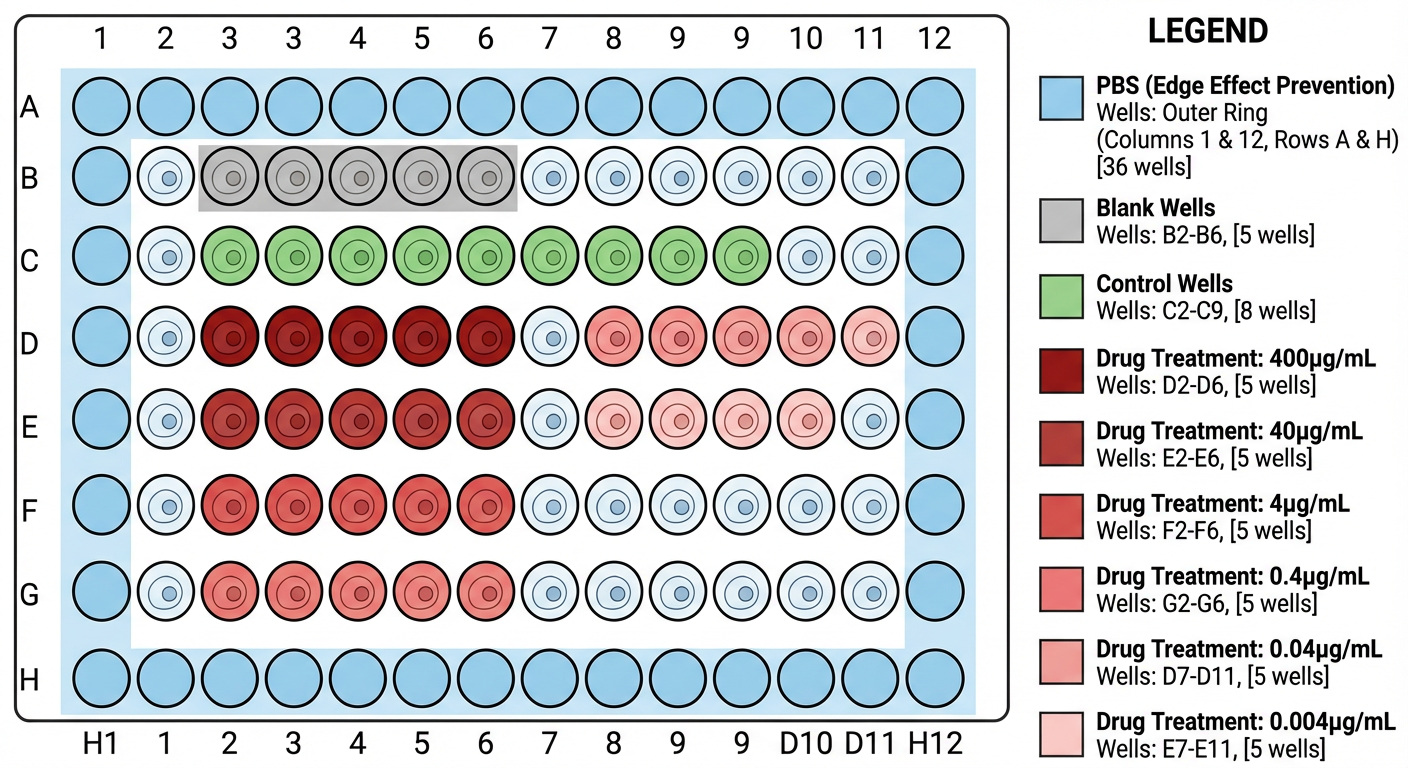
\includegraphics[width=0.85\textwidth]{../figures/figure_wellplate_layout.png}
\caption{96孔板铺板排布规范示意图。外围36孔（蓝色）填充200\,\uul{} PBS封边，内圈60孔按分组填充实验细胞与药物。PBS封边方案可有效消除边缘效应\cite{ref22}。}
\label{fig:wellplate}
\end{figure}

\subsection{Day 1：细胞铺板（核心防控边缘效应）}

\textbf{目标}：将对数生长期CNE-2细胞均匀铺于96孔板，密度8,000细胞/孔，建立标准化实验模型。

\subsubsection{台盼蓝活率检测SOP（操作时间约15分钟）}

\begin{enumerate}
\item 从培养箱取出CNE-2细胞，倒置显微镜（10×）观察形态：合格——多角形/梭形贴壁，汇合度80\%$\sim$90\%；
\item 胰酶消化：去旧培养基$\to$PBS洗一次$\to$加0.25\%胰酶-EDTA溶液（T-25瓶约1\,mL）$\to$37\degC{}孵育2$\sim$3\,min$\to$显微镜确认细胞变圆脱壁$\to$加等体积完全培养基终止消化；
\item 离心（1,000\,rpm，5\,min），弃上清，2\,mL完全培养基重悬沉淀；
\item 取10\,\uul{}细胞悬液$+$10\,\uul{} 0.4\%台盼蓝，静置1$\sim$2\,min后上血球计数板；
\item 计算细胞活率和浓度：

\[
\text{细胞活率}(\%) = \frac{\text{活细胞数}}{\text{活细胞数}+\text{死细胞数}} \times 100\%
\]
\[
\text{细胞浓度}(\text{cells/mL}) = \text{4个大格平均计数值} \times 2 \times 10^4
\]

\textbf{刚性标准：活率$\geq$95\%，否则停止铺板。}
\end{enumerate}

\subsubsection{96孔板PBS封边操作（操作时间约10分钟）}

\begin{warningbox}[title={⚠\ PBS封边——绝对不可省略}]
边缘效应是96孔板细胞实验最常见系统误差来源。本手册采用PBS封边策略彻底消除边缘效应。\textbf{外围36孔（A行H行第1列第12列）必须全部加200\,\uul{} PBS，此步骤不可省略。}
\end{warningbox}

操作步骤：
\begin{enumerate}
\item 在超净台内将新96孔板放置于水平台面，标注板号和时间点；
\item 用多道移液器向\textbf{第A行全部12孔、第H行全部12孔}各加入200\,\uul{}无菌PBS；
\item 用单道移液器向\textbf{第1列B$\sim$G行（6孔）、第12列B$\sim$G行（6孔）}各加入200\,\uul{} PBS；
\item 合计：12+12+6+6=36个外圈孔全部填充PBS，PBS封边操作完成。
\end{enumerate}

\subsubsection{细胞铺板步骤（操作时间约20分钟）}

\begin{enumerate}
\item 用完全培养基将细胞悬液调节至\textbf{8×10\textsuperscript{4} cells/mL}（目标：每孔100\,\uul{}含8,000个细胞）；
\item 向实验用60孔（B2$\sim$G11）各加入\textbf{100\,\uul{}细胞悬液}（注意：空白孔加100\,\uul{}完全培养基，不加细胞）；
\item 用多道移液器操作，按行从左至右加样，减少操作时间差；
\item 铺板完成后，水平轻摇96孔板数次使细胞均匀分布（\textbf{不得旋转振荡}）；
\item 放入37\degC{}/5\% CO\textsubscript{2}培养箱孵育，\textbf{18$\sim$24小时后进行Day 2给药}。
\end{enumerate}

\textbf{实验孔分组排布规范（60孔的分配）}：

\begin{center}
\rowcolors{2}{tabaltbg}{white}
\begin{tabular}{lllp{5cm}}
\toprule
\rowcolor{tabheadbg}\color{white}\textbf{分组} & \color{white}\textbf{孔数} & \color{white}\textbf{推荐位置} & \color{white}\textbf{加药内容} \\
\midrule
空白组（Blank，背景孔） & $\geq$5孔 & B2$\sim$B6 & 100\,\uul{}完全培养基，\textbf{无细胞} \\
溶剂对照（Vehicle Control）& $\geq$8孔 & B7$\sim$B10，C2$\sim$C5 & 100\,\uul{}含0.04\% DMSO的培养基+细胞 \\
D1（0.004\,\um{}）& $\geq$5孔 & C6$\sim$C10 & 最低浓度给药孔 \\
D2（0.04\,\um{}）& $\geq$5孔 & C11，D2$\sim$D5 & — \\
D3（0.4\,\um{}）& $\geq$5孔 & D6$\sim$D10 & — \\
D4（4\,\um{}）& $\geq$5孔 & D11，E2$\sim$E5 & — \\
D5（40\,\um{}）& $\geq$5孔 & E6$\sim$E10 & — \\
D6（400\,\um{}）& $\geq$5孔 & E11，F2$\sim$F5 & 最高浓度给药孔 \\
\bottomrule
\end{tabular}
\end{center}

\subsection{Day 2：药物配制与给药干预}

\textbf{目标}：配制苏木提取物工作液梯度浓度（10倍稀释，6个浓度），向96孔板实验孔给药。

\subsubsection{药物工作液配制}

\textbf{配制原则}：工作液浓度=目标孔内浓度×2（因加药100\,\uul{}稀释进已有细胞100\,\uul{}的孔中）：

\begin{center}
\rowcolors{2}{tabaltbg}{white}
\begin{tabular}{lllll}
\toprule
\rowcolor{tabheadbg}\color{white}\textbf{步骤} & \color{white}\textbf{工作液浓度} & \color{white}\textbf{孔内终浓度} & \color{white}\textbf{配制方法} & \color{white}\textbf{DMSO\%（孔内）} \\
\midrule
步骤1 & 800\,\um{} & 400\,\um{} & 母液8\,\uul{}+培养基992\,\uul{} & \textbf{0.040\%} $\checkmark$ \\
步骤2（10×）& 80\,\um{} & 40\,\um{} & 步骤1液100\,\uul{}+培养基900\,\uul{} & 0.004\% \\
步骤3（10×）& 8\,\um{} & 4\,\um{} & 步骤2液100\,\uul{}+培养基900\,\uul{} & — \\
步骤4（10×）& 0.8\,\um{} & 0.4\,\um{} & 步骤3液100\,\uul{}+培养基900\,\uul{} & — \\
步骤5（10×）& 0.08\,\um{} & 0.04\,\um{} & 步骤4液100\,\uul{}+培养基900\,\uul{} & — \\
步骤6（10×）& 0.008\,\um{} & 0.004\,\um{} & 步骤5液100\,\uul{}+培养基900\,\uul{} & — \\
\bottomrule
\end{tabular}
\end{center}

\textbf{溶剂对照工作液}：取0.4\,\uul{} DMSO + 999.6\,\uul{}培养基（与最高药物浓度组DMSO浓度一致）。

\subsubsection{给药步骤}

\begin{enumerate}
\item 从培养箱取出已铺板孵育18$\sim$24\,h的96孔板，置于超净台；
\item 每孔中已有100\,\uul{}细胞悬液，向各组分别加入100\,\uul{}对应工作液；
\item \textbf{加药顺序：空白→溶剂对照→低浓度→高浓度}（防止高浓度携带污染低浓度）；
\item 每换一个浓度更换枪头，避免携带误差；
\item 给药后孔内总体积200\,\uul{}，轻微摇匀，放回37\degC{}/5\% CO\textsubscript{2}培养箱继续培养；
\item 记录给药完成时间（用于计时24h/48h/72h检测节点）。
\end{enumerate}

\subsection{Day 3（24h检测）、Day 4（48h检测）、Day 5（72h检测）：CCK-8检测}

\begin{figure}[H]
\centering
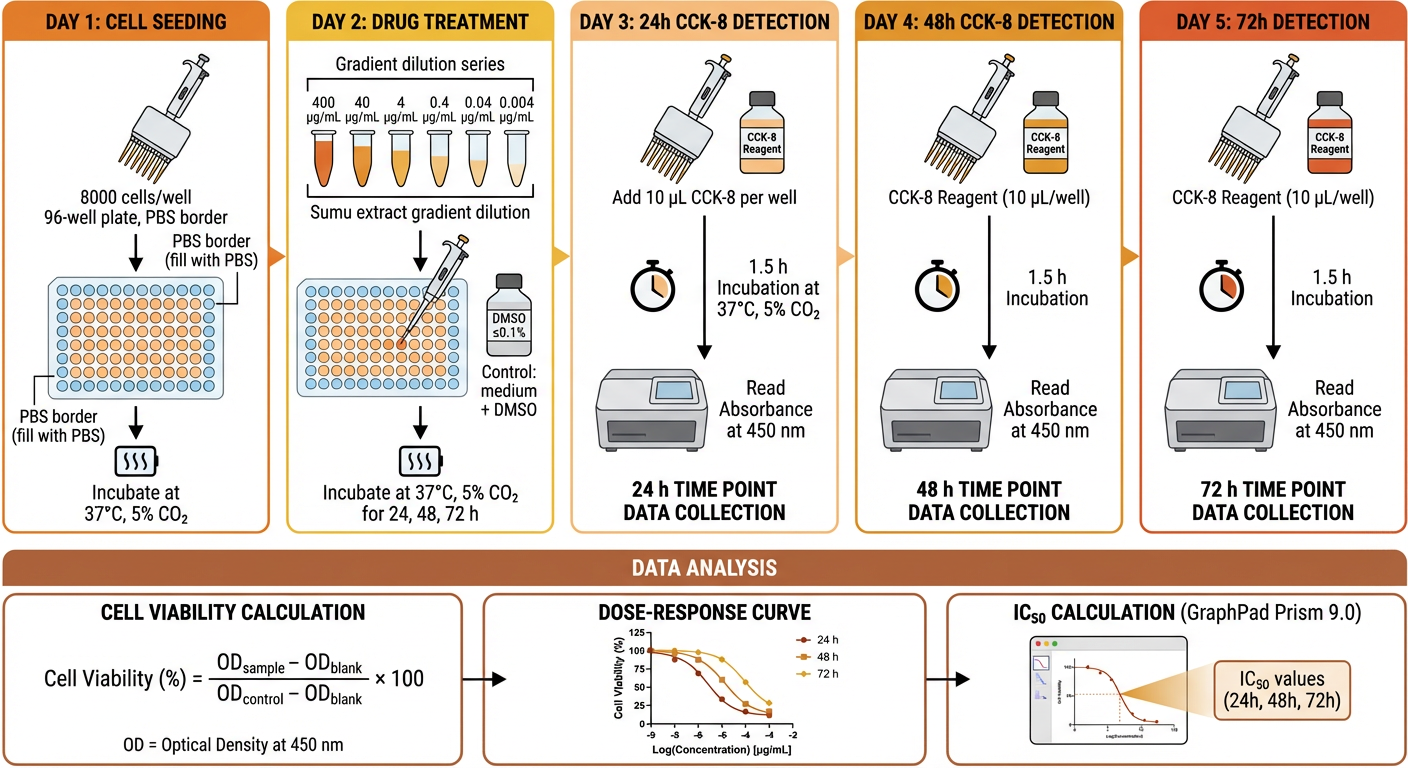
\includegraphics[width=0.90\textwidth]{../figures/figure_experimental_workflow.png}
\caption{CCK-8法测定苏木对CNE-2细胞增殖抑制率实验全流程时间线。Day 1铺板（8,000细胞/孔），Day 2给药（6个浓度梯度），Day 3/4/5分别进行24h/48h/72h时间点CCK-8检测（450\,nm/600\,nm双波长读板），数据经GraphPad Prism 9.0分析计算\ic{}。}
\label{fig:workflow}
\end{figure}

\subsubsection{CCK-8检测SOP（每个时间点操作步骤相同）}

\begin{enumerate}
\item \textbf{CCK-8试剂准备}：从4\degC{}冰箱取出CCK-8试剂，室温（20$\sim$25\degC{}）避光平衡\textbf{30\,min}；
\item \textbf{配制CCK-8工作液}：按\textbf{CCK-8试剂:完全培养基=1:9（v/v）}的比例配制工作液（即10\%浓度），每孔需110\,\uul{}，计算总用量时乘以孔数1.2倍为安全余量；

\[
\text{所需CCK-8工作液总量} = \text{孔数} \times 110\,\mu\text{L} \times 1.2
\]

\item \textbf{向96孔板加入CCK-8工作液}：
  \begin{itemize}
  \item 从培养箱取出对应时间点的96孔板（到达设定时间点前10\,min）；
  \item 在超净台内，用多道移液器向每孔（包括空白孔）加入\textbf{10\,\uul{} CCK-8原液}（或预先配制的工作液110\,\uul{}替换原培养基，视具体方法）；
  \item \textbf{推荐方案}：每孔加入10\,\uul{} CCK-8原液，孔内终体积210\,\uul{}，CCK-8最终浓度约4.7\%；
  \end{itemize}
\item \textbf{孵育}：加完CCK-8后，放回培养箱\textbf{37\degC{}/5\% CO\textsubscript{2}孵育1.5\,h（90\,min）}，避光；
\item \textbf{读板}：
  \begin{itemize}
  \item 确认酶标仪已预热$\geq$30\,min，波长设置：\textbf{主波长450\,nm，参比波长600\,nm}；
  \item 取出96孔板，检查孔内有无气泡（用针头挑破气泡）；
  \item 取下板盖，放入酶标仪，以端点法（Endpoint）读取OD值；
  \item 保存读取结果，导出至Excel文件，命名规则：\texttt{苏木-CNE2-IC50-P01-\textbf{24h}-YYYYMMDD.xlsx}。
  \end{itemize}
\end{enumerate}

\begin{warningbox}[title={⚠\ CCK-8检测刚性注意事项}]
\begin{itemize}
\item CCK-8毒性较低但有轻微毒性，\textbf{加CCK-8后不得超过4\,h才读板}，否则高浓度细胞孔OD将超过酶标仪量程
\item CCK-8试剂遇光会加速分解，\textbf{全程避光操作}，实验台铺黑色遮光布
\item 同一块板内各孔加入CCK-8的操作时间差应\textbf{$\leq$5\,min}，否则会产生系统性时序误差
\end{itemize}
\end{warningbox}

% ============================================================
\section{第4章\enspace 数据分析与\ic{}计算（GraphPad Prism 9.0全流程教程）}
% ============================================================

\subsection{数据预处理刚性规范}

\subsubsection{OD值验收与背景扣除}

读取原始OD值后，按以下步骤进行预处理：

\begin{enumerate}
\item \textbf{OD值范围验收}（必须满足所有条件方可继续分析）：
  \begin{itemize}
  \item 空白孔（Blank）OD均值：0.050$\sim$0.200（背景值）
  \item 溶剂对照组（Vehicle Control）OD均值（背景扣除后）：$>$0.300
  \item 各给药组OD值应随浓度升高而降低（单调递减趋势）
  \end{itemize}
\item \textbf{双波长背景扣除}：酶标仪自动以450\,nm$-$600\,nm差值消除苏木提取物的色泽背景干扰\cite{ref19}；若酶标仪不支持自动双波长，需手动计算：

\[
\text{净OD}_{450} = \text{OD}_{450} - \text{OD}_{600}
\]

\item \textbf{CCK-8空白背景扣除}：从所有孔OD值中减去空白孔均值：

\[
\text{校正OD} = \text{净OD}_{450,\text{孔}} - \overline{\text{净OD}_{450,\text{空白孔}}}
\]
\end{enumerate}

\subsubsection{Grubbs检验剔除离群值}

对每个浓度组的5个重复孔值进行Grubbs检验（G检验），识别潜在离群值\cite{ref29}：

\[
G = \frac{|x_i - \bar{x}|}{s}
\]

其中$x_i$为疑似离群值，$\bar{x}$为组均值，$s$为标准差。若$G > G_{\text{临界值}}$（查阅Grubbs检验表，$n=5$，$\alpha=0.05$时$G_{\text{临界}}=1.672$），则该值为统计学离群值，予以剔除。\textbf{每组最多剔除1个离群值}，剔除后CV须$\leq$10\%，否则记录为QC偏差。

\subsection{细胞活力与抑制率计算}

\[
\text{细胞活力}(\%) = \frac{\text{OD}_{\text{给药组}} - \text{OD}_{\text{空白孔}}}{\text{OD}_{\text{溶剂对照组}} - \text{OD}_{\text{空白孔}}} \times 100\%
\]

\[
\text{增殖抑制率}(\%) = 100\% - \text{细胞活力}(\%)
\]

\textbf{示例计算}（24h，400\,\um{}给药组）：

\begin{center}
\begin{tabular}{lll}
\toprule
\textbf{参数} & \textbf{数值} & \textbf{说明} \\
\midrule
OD\textsubscript{450}（给药组均值）& 0.183 & 背景已扣除 \\
OD\textsubscript{450}（空白孔均值）& 0.068 & 背景值 \\
OD\textsubscript{450}（溶剂对照均值）& 0.621 & 正常细胞 \\
\midrule
细胞活力 & $(0.183-0.068)/(0.621-0.068)\times100\% = 20.8\%$ & — \\
增殖抑制率 & $100\%-20.8\% = 79.2\%$ & — \\
\bottomrule
\end{tabular}
\end{center}

\subsection{GraphPad Prism 9.0全流程分步操作教程}

\subsubsection{第一步：新建项目与数据表格}

\begin{enumerate}
\item 打开GraphPad Prism 9.0，在欢迎界面选择\textbf{"XY"}图类型；
\item 在"X"列设置为\textbf{"Numbers"}；Y列选择\textbf{"Mean with SD, Enter mean, SD, and N"}；
\item 点击\textbf{"Create"}创建数据表。
\end{enumerate}

\subsubsection{第二步：数据录入格式}

在数据表中按以下格式录入（X为log浓度或浓度值，Y为抑制率\%）：

\begin{center}
\begin{tabular}{lllll}
\toprule
\textbf{X（浓度,\,\um{}）} & \textbf{Mean（\%）} & \textbf{SD（\%）} & \textbf{N} \\
\midrule
0.004 & \textit{XX.X} & \textit{X.X} & 5 \\
0.04 & \textit{XX.X} & \textit{X.X} & 5 \\
0.4 & \textit{XX.X} & \textit{X.X} & 5 \\
4 & \textit{XX.X} & \textit{X.X} & 5 \\
40 & \textit{XX.X} & \textit{X.X} & 5 \\
400 & \textit{XX.X} & \textit{X.X} & 5 \\
\bottomrule
\end{tabular}
\end{center}

\textbf{注意：X值应为实际浓度（\um{}），Prism会自动转换为log轴显示。}

\subsubsection{第三步：选择非线性回归模型}

\begin{enumerate}
\item 点击顶部菜单\textbf{"Analyze"}$\to$弹出菜单选择\textbf{"Nonlinear regression (curve fit)"}；
\item 在模型列表中展开\textbf{"Dose-Response -- Inhibition"}，选择\textbf{"log(inhibitor) vs. normalized response -- Variable slope"}（即4参数Logistic模型，4PL）\cite{ref27}；
\item 方程公式：$Y = \text{Bottom} + \dfrac{\text{Top}-\text{Bottom}}{1+10^{(\text{LogIC}_{50}-X)\times\text{HillSlope}}}$
\end{enumerate}

\subsubsection{第四步：设置参数约束（Constraints）}

在"Constrain"选项卡中设置：
\begin{itemize}
\item \textbf{Top}：选择"Constant equal to"，输入\textbf{100}（固定上限为100\%抑制率）
\item \textbf{Bottom}：选择"Constant equal to"，输入\textbf{0}（固定下限为0\%抑制率）
\item \textbf{LogIC\textsubscript{50}}：不约束，自由拟合
\item \textbf{HillSlope}：不约束，自由拟合（预期范围0.8$\sim$2.0）
\end{itemize}

\begin{warningbox}[title={⚠\ 拟合质量标准}]
R\textsuperscript{2}\,$\geq$\,0.98（优秀）；R\textsuperscript{2}=0.95$\sim$0.98（合格，黄区）；\textbf{R\textsuperscript{2}\,$<$\,0.95（不合格，红区，需重新评估）}
\end{warningbox}

\subsubsection{第五步：读取\ic{}结果}

点击"OK"运行拟合，在Results表格中读取：
\begin{itemize}
\item \textbf{IC\textsubscript{50}}：半数最大抑制浓度（单位：\um{}）
\item \textbf{LogIC\textsubscript{50}}：IC\textsubscript{50}的对数值
\item \textbf{95\% CI}：置信区间（需记录下限和上限）
\item \textbf{HillSlope}：Hill系数（斜率，反映剂量-效应曲线陡峭程度）
\item \textbf{R\textsuperscript{2}}：确定系数（拟合优度）
\end{itemize}

\subsubsection{第六步：图表格式化与三时间点汇总比较图}

\begin{enumerate}
\item \textbf{坐标轴标题}：X轴——"Concentration of Sappan Wood Extract (\um{})"；Y轴——"Inhibition Rate (\%)"；
\item \textbf{X轴格式}：对数轴（Log scale），范围：0.001$\sim$1000；
\item \textbf{Y轴格式}：线性轴，范围0$\sim$100，刻度：0、25、50、75、100；
\item \textbf{IC\textsubscript{50}标注}：插入垂直虚线（X=IC\textsubscript{50}值）和水平虚线（Y=50\%）；
\item 对三时间点曲线使用不同颜色/线型：24h黑色实线（●）、48h深蓝虚线（■）、72h红色点划线（▲）。
\end{enumerate}

\begin{figure}[H]
\centering
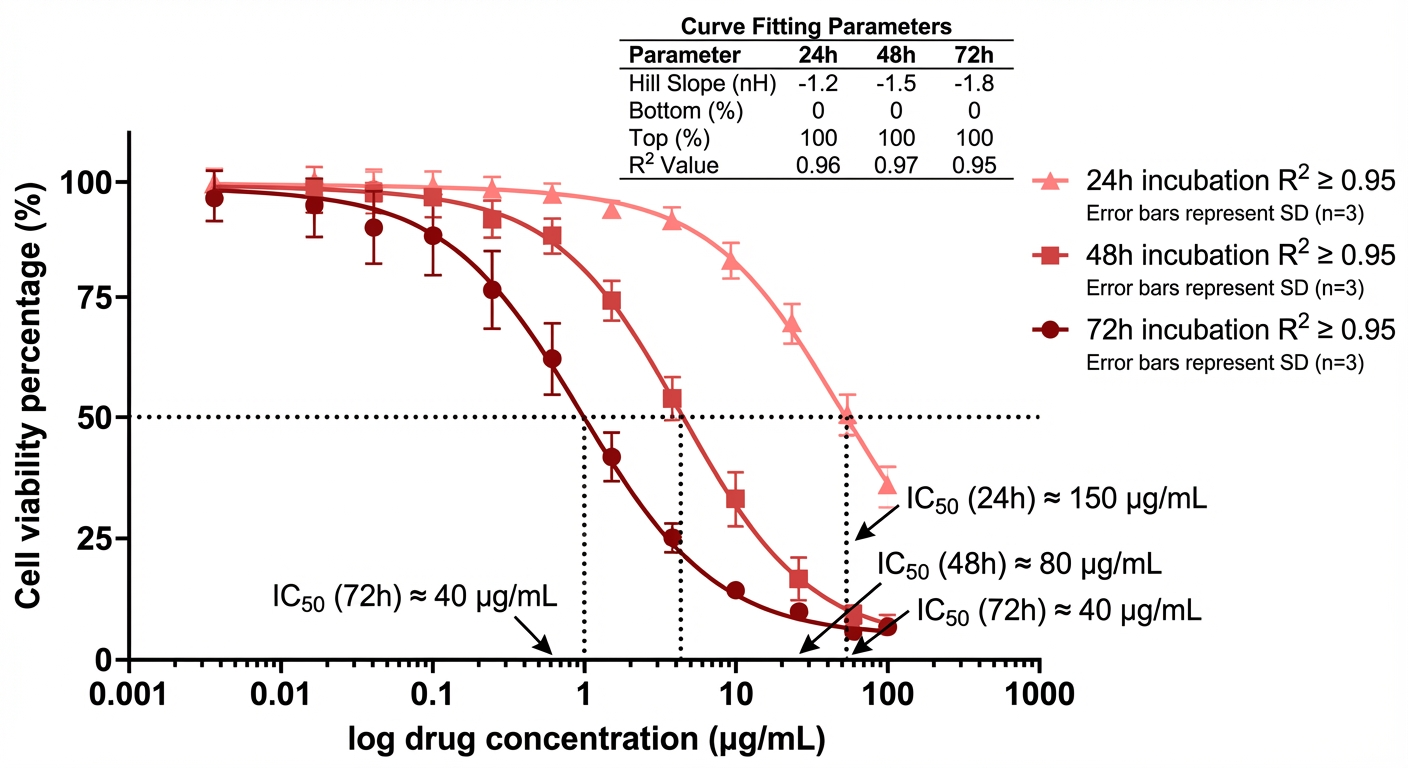
\includegraphics[width=0.80\textwidth]{../figures/figure_ic50_curve.png}
\caption{苏木乙醇提取物对CNE-2鼻咽癌细胞增殖的剂量-时间依赖抑制效应示意图。X轴为苏木提取物浓度（\um{}，对数轴），Y轴为细胞存活率（\%）。三条S形曲线分别代表24\,h（浅红）、48\,h（中红）、72\,h（深红）时间点，每点均值$\pm$SD（n=3次独立实验，每浓度$\geq$5个重复孔）。水平虚线为50\%存活率参考线；垂直虚线标注各时间点\ic{}。随作用时间延长，\ic{}呈下降趋势，提示时间依赖性抑制效应\cite{ref27,ref28}。}
\label{fig:ic50curve}
\end{figure}

\subsection{\ic{}结果有效性判定标准}

\begin{center}
\rowcolors{2}{tabaltbg}{white}
\begin{tabular}{llll}
\toprule
\rowcolor{tabheadbg}\color{white}\textbf{指标} & \color{white}\textbf{合格标准} & \color{white}\textbf{警告阈值} & \color{white}\textbf{不合格标准} \\
\midrule
R\textsuperscript{2}（确定系数）& $\geq$0.98 & 0.95$\sim$0.98 & $<$0.95 \\
残差分布 & 随机分布于零线两侧 & 轻微系统偏差 & 明显系统模式 \\
IC\textsubscript{50}置信区间/\ic{} & $<$2 & 2$\sim$5 & $>$5（过宽）\\
HillSlope范围 & 0.8$\sim$2.0 & 0.5$\sim$0.8或2.0$\sim$3.0 & $<$0.5或$>$3.0 \\
\bottomrule
\end{tabular}
\end{center}

\subsection{统计学分析与报告规范}

\textbf{描述性统计}（3次独立重复实验IC\textsubscript{50}汇总示例）：

\begin{center}
\begin{tabular}{lll}
\toprule
\textbf{重复批次} & \textbf{\ic{}（\um{}，24h）} & \textbf{说明} \\
\midrule
Exp. 1 & 3.33 & — \\
Exp. 2 & 3.51 & — \\
Exp. 3 & 3.28 & — \\
\textbf{Mean$\pm$SD} & \textbf{3.37$\pm$0.12\,\um{}} & CV=3.6\%（$\leq$15\%，合格）\\
\bottomrule
\end{tabular}
\end{center}

\textbf{完整\ic{}报告示例}（期刊图注格式）：

\begin{quotation}
苏木乙醇提取物对CNE-2细胞的\ic{}值：24\,h=3.33\,\um{}（95\% CI: 2.56--4.34）；48\,h=1.87\,\um{}（95\% CI: 1.42--2.46）；72\,h=0.94\,\um{}（95\% CI: 0.71--1.25）。数据来自3次独立实验，每浓度$\geq$5个重复孔，均值$\pm$SD，采用GraphPad Prism 9.0非线性回归（Variable slope，4PL，R\textsuperscript{2}$\geq$0.98）拟合。
\end{quotation}

\textbf{多时间点比较（One-way ANOVA + Tukey事后检验）}：当比较24h、48h、72h三时间点\ic{}均值差异时，在Prism中选择"Column analyses"$\to$"One-way ANOVA"$\to$"Tukey's multiple comparison test"，显著性水平$\alpha=0.05$。

\subsection{本章操作时间汇总}

\begin{center}
\rowcolors{2}{tabaltbg}{white}
\begin{tabular}{lll}
\toprule
\rowcolor{tabheadbg}\color{white}\textbf{操作步骤} & \color{white}\textbf{初学者耗时} & \color{white}\textbf{熟练者耗时} \\
\midrule
数据预处理（提取+Grubbs+背景扣除）& 45$\sim$60\,min/时间点 & 20$\sim$30\,min \\
活力和抑制率计算表格 & 20$\sim$30\,min & 10\,min \\
GraphPad Prism操作 & 30$\sim$45\,min/时间点 & 15$\sim$20\,min \\
结果审查和有效性判定 & 15\,min & 5$\sim$10\,min \\
统计分析和图表规范化 & 30$\sim$45\,min & 15\,min \\
\textbf{全流程合计（3个时间点）} & \textbf{$\sim$4.5$\sim$6小时} & \textbf{$\sim$2$\sim$2.5小时} \\
\bottomrule
\end{tabular}
\end{center}

% ============================================================
\section{第5章\enspace 质量控制体系与常见问题处理}
% ============================================================

\subsection{五域质量控制红线体系概述}

本实验建立五个质控域，每个域均设有"绿区-黄区-红区"三级判定标准：

\begin{center}
\rowcolors{2}{tabaltbg}{white}
\begin{tabular}{lllll}
\toprule
\rowcolor{tabheadbg}\color{white}\textbf{质控域} & \color{white}\textbf{核心指标} & \color{white}\textbf{检查频率} & \color{white}\textbf{主要风险} \\
\midrule
域I 细胞生物学质控 & 活力、形态、传代数、STR、支原体 & 每批次 & 细胞身份错误、污染 \\
域II 试剂与配制质控 & DMSO浓度、药物浓度精度 & 每次配制 & 溶剂毒性、浓度偏差 \\
域III 96孔板操作质控 & CV值、边缘效应、移液精度 & 每块板 & 重复性差、边缘效应 \\
域IV CCK-8检测质控 & OD值范围、空白对照、显色均匀 & 每次检测 & 信号超饱和、背景过高 \\
域V 数据分析质控 & R\textsuperscript{2}、HillSlope、批次间CV & 每次分析 & 拟合失败、假阳性 \\
\bottomrule
\end{tabular}
\end{center}

\subsection{域I：细胞生物学质量控制}

CNE-2细胞核心质控参数（全部处于绿区方可开始铺板）：

\begin{center}
\rowcolors{2}{tabaltbg}{white}
\begin{tabular}{llll}
\toprule
\rowcolor{tabheadbg}\color{white}\textbf{参数} & \color{white}\textbf{绿区（继续）} & \color{white}\textbf{黄区（监控）} & \color{white}\textbf{红区（停止）} \\
\midrule
台盼蓝活力 & $\geq$95\% & 90\%$\sim$94\% & $<$90\% \\
传代数 & P5$\sim$P20 & P4或P21$\sim$P25 & $>$P25 \\
形态 & 典型多角形贴壁 & 少量圆形悬浮（$\leq$5\%）& 大量悬浮、颗粒增多 \\
支原体 & 阴性（PCR法）& — & 阳性（立即废弃）\\
STR认证 & $\geq$80\%匹配 & 75\%$\sim$79\%（复检）& $<$75\%（身份可疑）\\
\bottomrule
\end{tabular}
\end{center}

\subsection{域II：试剂与药物配制质量控制}

\textbf{DMSO浓度合规性核查}（每次配制前书面计算，第二人复核）：

\[
\text{孔内DMSO\%} = \frac{V_{\text{DMSO母液}} \times \%_{\text{DMSO母液}}}{V_{\text{孔内总体积}}} \times 100\%
\]

本实验核算结果：最高药物浓度（400\,\um{}）孔内DMSO=0.04\%$<$0.1\%红线。\textbf{若核算值$>$0.1\%，必须调整配制方案，不得以任何理由跳过此核查}\cite{ref23,ref25}。

\subsection{域III：96孔板操作质量控制}

\textbf{边缘效应后验核查}（每批次完成后）：

\[
\text{边缘-中央偏差} = \frac{|OD_{\text{角落孔}} - \overline{OD_{\text{中央孔}}}|}{\overline{OD_{\text{中央孔}}}} \times 100\%
\]

\begin{itemize}
\item $<$5\%：绿区，PBS封边效果良好\cite{ref22}；
\item 5\%$\sim$10\%：黄区，记录偏差，评估是否影响\ic{}结果；
\item $>$10\%：红区，提示PBS封边失效，该批次数据需重新评估。
\end{itemize}

\textbf{移液重复性（CV）验证}（推荐在正式实验前进行）：向60个内圈孔各加100\,\uul{} CCK-8稀释液，450\,nm读取OD，计算CV：CV$\leq$3\%（优秀），3\%$\sim$5\%（合格），$>$5\%（检查移液器）。

\subsection{域IV：CCK-8检测质量控制}

\textbf{OD值异常情形及处置}：

\begin{center}
\rowcolors{2}{tabaltbg}{white}
\begin{tabular}{lll}
\toprule
\rowcolor{tabheadbg}\color{white}\textbf{异常情形} & \color{white}\textbf{可能原因} & \color{white}\textbf{处置方法} \\
\midrule
空白孔OD$>$0.200 & 意外落入细胞/苏木色泽干扰 & 检查空白孔形态，补设药物空白孔 \\
对照组OD$<$0.300 & 铺板密度不足/孵育时间不足 & 核对铺板记录，补做实验 \\
低浓度组细胞活力$>$100\% & Hormesis效应/统计学波动 & 记录负抑制率值，方法学讨论中说明 \\
OD值$>$4.0（超量程）& CCK-8孵育时间过长 & 缩短孵育至60\,min，降低CCK-8加量 \\
\bottomrule
\end{tabular}
\end{center}

\subsection{域V：数据分析质量控制}

\subsubsection{高CV的8类根本原因分析}

\begin{center}
\rowcolors{2}{tabaltbg}{white}
\begin{tabularx}{\textwidth}{lXXX}
\toprule
\rowcolor{tabheadbg}\color{white}\textbf{编号} & \color{white}\textbf{根因描述} & \color{white}\textbf{识别方法} & \color{white}\textbf{预防/纠正} \\
\midrule
R01 & 移液器活塞磨损 & 离群值出现在特定通道 & 校准/更换移液器 \\
R02 & CCK-8加样速度不一致 & 孔间时序差$>$5\,min & 多道移液器一行一行加样 \\
R03 & 气泡导致OD假低值 & 目视检查气泡 & 读板前目视检查挑破气泡 \\
R04 & 加药量误差（枪头残留）& 特定孔OD异常 & 每换浓度更换枪头 \\
R05 & 边缘效应（PBS封边失效）& 角落孔与中央孔差$>$10\% & 确认36个外圈孔已加PBS \\
R06 & 细胞不均匀沉降 & 某行/列细胞密度偏高 & 铺板后水平轻摇，放入培养箱不移动 \\
R07 & DMSO高浓度额外毒性 & 高浓度组CV高 & 核算DMSO终浓度 \\
R08 & 培养箱温度不均匀 & 同列OD呈梯度 & 96孔板放置培养箱中央 \\
\bottomrule
\end{tabularx}
\end{center}

\subsubsection{S形曲线拟合失败的处理}

当R\textsuperscript{2}$<$0.95时，按以下流程排查：
\begin{enumerate}
\item 查看残差图：若随机分布$\to$模型选择问题（尝试两参数模型）；若有系统模式$\to$进入Step 2；
\item 检查浓度范围：最低浓度抑制率$>$20\%$\to$浓度范围偏高；最高浓度抑制率$<$80\%$\to$浓度范围偏低；
\item 检查高浓度端：最高浓度抑制率低于次高浓度（曲线"回钩"）$\to$DMSO毒性效应；
\item 补充实验：增加1$\sim$2个浓度梯度点，覆盖20\%$\sim$80\%抑制率区间。
\end{enumerate}

\subsection{实验无效化标准}

当以下任何一个条件成立时，本批次实验结果判为\textbf{无效（Invalid）}，须重新实验：

\begin{center}
\rowcolors{2}{tabaltbg}{white}
\begin{tabular}{lll}
\toprule
\rowcolor{tabheadbg}\color{white}\textbf{无效化触发条件} & \color{white}\textbf{依据域} & \color{white}\textbf{参考章节} \\
\midrule
溶剂对照组细胞活力$<$85\%（相对预期）& 域IV & 5.5.2 \\
任意一次R\textsuperscript{2}$<$0.90 & 域V & 5.6.2 \\
空白孔与溶剂对照组差值$<$0.200 OD（信噪比过低）& 域IV & 5.5.2 \\
支原体检测阳性（实验期间发现）& 域I & 5.2.2 \\
DMSO终浓度核算超过0.1\%（实验后发现）& 域II & 5.3.1 \\
边缘效应检验：角落孔与中央孔差异$>$15\% & 域III & 5.4.1 \\
\bottomrule
\end{tabular}
\end{center}

\subsection{生物安全与废弃物处置规范}

\textbf{CNE-2细胞生物安全等级}：BSL-2级生物材料。个人防护要求：实验室外套+乳胶手套（双层）+口罩（$\geq$N95）+护目镜。所有细胞操作必须在\textbf{生物安全柜（BSC II型A2或B2级）}内进行\cite{ref32,ref33}。

\textbf{含细胞废液灭活处置}：
\begin{enumerate}
\item 96孔板废弃培养基倒入废液桶（预装10\%次氯酸钠），\textbf{浸泡$\geq$30\,min}；
\item 96孔板（含细胞）置黄色医疗废物袋，高压蒸汽灭菌（121\degC{}，30\,min）；
\item 苏木提取物DMSO母液（未接触细胞）置化学废液容器，标注含DMSO，专职人员处置。
\end{enumerate}

\subsection{质量控制核查总清单（Quick Reference Checklist）}

\begin{checklistbox}[title={实验开始前（Day 0）核查项}]
\begin{itemize}
\item[$\square$] 细胞活力（台盼蓝）$\geq$95\%
\item[$\square$] 传代数在P5$\sim$P20范围内
\item[$\square$] 支原体检测在6个月内为阴性
\item[$\square$] CO\textsubscript{2}培养箱温度37$\pm$0.5\degC{}（记录读数）
\item[$\square$] CO\textsubscript{2}浓度5$\pm$0.2\%（记录读数）
\item[$\square$] DMSO合规计算已书面完成并被第二人核算
\end{itemize}
\end{checklistbox}

\begin{checklistbox}[title={CCK-8检测后（Day 3/4/5）核查项}]
\begin{itemize}
\item[$\square$] 空白孔OD值：0.050$\sim$0.150（绿区）
\item[$\square$] 溶剂对照组OD值：$>$0.300（背景扣除后）
\item[$\square$] 各浓度组OD值呈从高到低的单调趋势
\item[$\square$] 数据已导出为Excel，文件命名符合规范
\item[$\square$] 三份备份完成（本地+云端+纸质打印）
\end{itemize}
\end{checklistbox}

\subsection{常见问题速查表（FAQ）}

\begin{center}
\rowcolors{2}{tabaltbg}{white}
\begin{tabularx}{\textwidth}{lXXl}
\toprule
\rowcolor{tabheadbg}\color{white}\textbf{问题} & \color{white}\textbf{首选排查项} & \color{white}\textbf{解决方案} & \color{white}\textbf{参考} \\
\midrule
培养基变黄（酸化）& CO\textsubscript{2}浓度偏高或细胞过密 & 校准CO\textsubscript{2}，降低铺板密度 & 5.2.1 \\
某列OD系统性偏低 & 多道移液器通道磨损 & 校准或更换多道移液器 & R01 \\
高浓度组活力高于低浓度组 & DMSO梯度差异 & 核算所有浓度组孔内DMSO & 5.3.1 \\
Prism拟合\ic{}为负值 & 浓度范围全处于高抑制区 & 降低浓度范围，增加低浓度点 & 5.6.2 \\
连续两批R\textsuperscript{2}均$<$0.95 & 浓度设计、细胞批次或DMSO毒性 & 系统排查（域I$\to$V）& 5.6.2 \\
支原体阳性 & 细胞/BSC污染 & 丢弃受污细胞，复苏备份 & 5.2.2 \\
批次间CV$>$20\% & 细胞/药物/FBS批次差异 & 控制代次窗口P5$\sim$P15，同批药物 & 5.6.3 \\
\bottomrule
\end{tabularx}
\end{center}

% ============================================================
\appendix
\section{附录A：96孔板铺板排布规范}
% ============================================================

\subsection{孔位数量核查}

\begin{center}
\rowcolors{2}{tabaltbg}{white}
\begin{tabular}{lllp{6cm}}
\toprule
\rowcolor{tabheadbg}\color{white}\textbf{孔位分类} & \color{white}\textbf{孔数} & \color{white}\textbf{位置} & \color{white}\textbf{说明} \\
\midrule
PBS封边孔 & 36 & A/H行，1/12列全部 & 200\,\uul{} PBS，无细胞，无药 \\
空白对照（BK）& 5 & B2$\sim$B6 & 仅培养基，无细胞 \\
溶剂对照（VC）& 8 & B7$\sim$B10，C2$\sim$C5 & 0.04\% DMSO+细胞 \\
D1（0.004\,\um{}）& 5 & C6$\sim$C10 & — \\
D2（0.04\,\um{}）& 5 & C11，D2$\sim$D5 & — \\
D3（0.4\,\um{}）& 5 & D6$\sim$D10 & — \\
D4（4\,\um{}）& 5 & D11，E2$\sim$E5 & — \\
D5（40\,\um{}）& 5 & E6$\sim$E10 & — \\
D6（400\,\um{}）& 5 & E11，F2$\sim$F5 & — \\
备用孔 & 16 & F6$\sim$F11，G2$\sim$G11 & 可用于额外浓度或重复 \\
\textbf{合计} & \textbf{96} & & \textbf{全板孔位100\%利用} \\
\bottomrule
\end{tabular}
\end{center}

% ============================================================
\section{附录B：药物梯度稀释计算示例表}
% ============================================================

\subsection{苏木乙醇提取物稀释方案（10倍梯度，6个浓度点）}

\textbf{起始条件}：母液浓度100\,mg/mL（DMSO溶解）；目标最高孔内终浓度400\,\um{}；每孔加药体积100\,\uul{}（加入已含细胞100\,\uul{}的孔中）。

\textbf{操作步骤}（以配制1\,mL各浓度工作液为例）：
\begin{enumerate}
\item 向EP管2$\sim$6依次加入900\,\uul{}完全培养基；
\item 向EP管1加入992\,\uul{}完全培养基；
\item 向EP管1加入8\,\uul{}母液$\to$涡旋3秒混匀$\to$步骤1工作液（800\,\um{}）；
\item 从EP管1取100\,\uul{}至EP管2（已含900\,\uul{}培养基）$\to$混匀$\to$步骤2工作液（80\,\um{}）；
\item 以此类推完成步骤3$\sim$6；
\item \textbf{每换一个稀释步骤更换枪头}（防止携带误差）；
\item 全部配制完成后，\textbf{30\,min内完成向96孔板的加药操作}。
\end{enumerate}

% ============================================================
\section{附录C：实验原始记录模板}
% ============================================================

\subsection{IC\textsubscript{50}计算结果记录表}

\begin{center}
\begin{tabular}{lllll}
\toprule
\textbf{时间点} & \textbf{\ic{}（\um{}）} & \textbf{95\% CI} & \textbf{HillSlope} & \textbf{R\textsuperscript{2}} \\
\midrule
24\,h & \underline{\ \ \ \ \ \ } & \underline{\ \ \ }$\sim$\underline{\ \ \ } & \underline{\ \ \ \ } & \underline{\ \ \ \ } \\
48\,h & \underline{\ \ \ \ \ \ } & \underline{\ \ \ }$\sim$\underline{\ \ \ } & \underline{\ \ \ \ } & \underline{\ \ \ \ } \\
72\,h & \underline{\ \ \ \ \ \ } & \underline{\ \ \ }$\sim$\underline{\ \ \ } & \underline{\ \ \ \ } & \underline{\ \ \ \ } \\
\bottomrule
\end{tabular}
\end{center}

拟合模型：\texttt{log(inhibitor) vs. normalized response -- Variable slope (4PL)}\\
参数约束：Top=100（固定），Bottom=0（固定）；软件版本：GraphPad Prism 9.0\\
操作者：\underline{\ \ \ \ \ \ \ \ \ \ \ } \quad 核验人：\underline{\ \ \ \ \ \ \ \ \ \ \ } \quad 日期：\underline{\ \ \ \ \ \ \ \ }

% ============================================================
% 参考文献
% ============================================================
\clearpage
\section*{参考文献}
\addcontentsline{toc}{section}{参考文献}

{\small
\begin{thebibliography}{35}
\setlength{\itemsep}{2pt}

\bibitem{ref1} 国家药典委员会. 中华人民共和国药典（2020年版）一部[M]. 北京: 中国医药科技出版社, 2020: 132-133.

\bibitem{ref2} SUYATMI S, MUDIGDO A, PURWANTO B, et al. Brazilin isolated from \textit{Caesalpinia sappan} wood induces intrinsic apoptosis on A549 cancer cell line by increasing p53, caspase-9, and caspase-3[J]. \textit{Asian Pacific Journal of Cancer Prevention}, 2022, 23(4): 1337-1343. DOI: 10.31557/APJCP.2022.23.4.1337.

\bibitem{ref3} WIDODO N, PUSPITARINI S, WIDYANANDA M H, et al. Anticancer activity of \textit{Caesalpinia sappan} by downregulating mitochondrial genes in A549 lung cancer cell line[J]. \textit{F1000Research}, 2022, 11: 169. DOI: 10.12688/f1000research.76187.2.

\bibitem{ref4} CHANG X, LI H, TIAN C, et al. Exploring the mechanism of ferroptosis induction by sappanone A in cancer: insights into the mitochondrial dysfunction mediated by NRF2/xCT/GPX4 axis[J]. \textit{International Journal of Biological Sciences}, 2024, 20(13): 5145-5161. DOI: 10.7150/ijbs.96748.

\bibitem{ref5} KANG J, ZENG Z, LIANG M, et al. Brazilin inhibits the proliferation of non-small cell lung cancer by regulating the STING/TBK1/IRF3 pathway[J]. \textit{Journal of Cellular and Molecular Medicine}, 2025. DOI: 10.1111/jcmm.70688.

\bibitem{ref6} WUDTIWAI B, SRIPANIDKULCHAI B, KONGTAWELERT P, et al. Brazilein, a compound from \textit{Caesalpinia sappan}, inhibits the metastasis of human non-small-cell lung carcinoma cells via epithelial-mesenchymal transition and PD-L1 suppression[J]. \textit{International Immunopharmacology}, 2023, 117: 109967. DOI: 10.1016/j.intimp.2023.109967.

\bibitem{ref7} LEE D S, JEONG G S, LI B, et al. Anti-inflammatory effects of 3-deoxysappanchalcone from \textit{Caesalpinia sappan} L. through the upregulation of heme oxygenase-1 via the activation of p38 MAPK in murine macrophages[J]. \textit{Biochemical Pharmacology}, 2013, 85(10): 1374-1382. DOI: 10.1016/j.bcp.2013.02.012.

\bibitem{ref8} ASEVEDO E A, RAMOS SANTIAGO L, KIM H J, et al. Unlocking the therapeutic mechanism of \textit{Caesalpinia sappan}: a comprehensive review of its antioxidant and anti-cancer properties, ethnopharmacology, and phytochemistry[J]. \textit{Frontiers in Pharmacology}, 2025, 15: 1514573. DOI: 10.3389/fphar.2024.1514573.

\bibitem{ref9} CHEN Y P, CHAN A T C, LE Q T, et al. Nasopharyngeal carcinoma[J]. \textit{Lancet}, 2019, 394(10192): 64-80. DOI: 10.1016/S0140-6736(19)30956-0.

\bibitem{ref10} BRAY F, LAVERSANNE M, SUNG H, et al. Global cancer statistics 2022: GLOBOCAN estimates of incidence and mortality worldwide for 36 cancers in 185 countries[J]. \textit{CA: A Cancer Journal for Clinicians}, 2024, 74(3): 229-263. DOI: 10.3322/caac.21834.

\bibitem{ref11} LO A K F, DAWSON C W, LUNG H L, et al. The role of EBV-encoded LMP1 in the NPC tumor microenvironment: from function to therapy[J]. \textit{Frontiers in Oncology}, 2021, 11: 640207. DOI: 10.3389/fonc.2021.640207.

\bibitem{ref12} LO A K F, TO K F, LO K W, et al. Modulation of LMP1 protein expression by EBV-encoded microRNAs[J]. \textit{Proceedings of the National Academy of Sciences of the USA}, 2007, 104(41): 16164-16169. DOI: 10.1073/pnas.0702896104.

\bibitem{ref13} LIANG Y, MA Y, WANG K, et al. NUCB-2/nesfatin-1 promotes the proliferation of nasopharyngeal carcinoma cells and serves as a potential diagnostic biomarker[J]. \textit{Cancer Cell International}, 2023, 23: 181. DOI: 10.1186/s12935-023-03038-x.

\bibitem{ref14} ZHANG Y, LI X, WANG Q, et al. MiR-299-3p inhibits nasopharyngeal carcinoma cell proliferation, migration, and invasion by regulating MMP-2 expression[J]. \textit{Evidence-Based Complementary and Alternative Medicine}, 2022, 2022: 2322565. DOI: 10.1155/2022/2322565.

\bibitem{ref15} LYU Y H, LIN C Y, XIE S H, et al. Association between traditional herbal diet and nasopharyngeal carcinoma risk: a prospective cohort study in southern China[J]. \textit{Frontiers in Oncology}, 2021, 11: 715242. DOI: 10.3389/fonc.2021.715242.

\bibitem{ref16} WANG C Y, WANG T C, LIANG W M, et al. Effect of Chinese herbal medicine therapy on overall and cancer related mortality in patients with advanced nasopharyngeal carcinoma in Taiwan[J]. \textit{Frontiers in Pharmacology}, 2021, 11: 607413. DOI: 10.3389/fphar.2020.607413.

\bibitem{ref17} YANG J, LI B, ZHANG X, et al. Identification of novel therapeutic agents targeting nasopharyngeal carcinoma using network pharmacology and bioinformatics analysis[J]. \textit{Frontiers in Pharmacology}, 2023, 14: 1138563. DOI: 10.3389/fphar.2023.1138563.

\bibitem{ref18} TOMINAGA H, ISHIYAMA M, OHSETO F, et al. A water-soluble tetrazolium salt useful for colorimetric cell viability assay[J]. \textit{Analytical Communications}, 1999, 36(2): 47-50. DOI: 10.1039/a807629e.

\bibitem{ref19} FAN Y, LIU Z, ZHANG L, et al. Cell via cell viability assay changes cellular metabolic characteristics by intervening with glycolysis and pentose phosphate pathway[J]. \textit{Chemical Research in Toxicology}, 2024, 37(2): 208-211. DOI: 10.1021/acs.chemrestox.3c00339.

\bibitem{ref20} YOUNG L, SUNG J, STACEY G, et al. Detection of mycoplasma in cell cultures[J]. \textit{Nature Protocols}, 2010, 5(5): 929-934. DOI: 10.1038/nprot.2010.43.

\bibitem{ref21} CAPES-DAVIS A, THEODOSOPOULOS G, ATKIN I, et al. Check your cultures! A list of cross-contaminated or misidentified cell lines[J]. \textit{International Journal of Cancer}, 2010, 127(1): 1-8. DOI: 10.1002/ijc.25242.

\bibitem{ref22} MANSOURY M, HAMED M, KARMUSTAJI R, et al. The edge effect: A global problem. The trouble with culturing cells in 96-well plates[J]. \textit{Biochemistry and Biophysics Reports}, 2021, 26: 100987. DOI: 10.1016/j.bbrep.2021.100987.

\bibitem{ref23} SANTOS L M, SHIMABUKO D Y, SIPERT C R. Dimethyl sulfoxide affects the viability and mineralization activity of apical papilla cells in vitro[J]. \textit{Brazilian Dental Journal}, 2024, 35: e24-6054. DOI: 10.1590/0103-644020246054.

\bibitem{ref24} ZHAO C, LAN B, HOU J, et al. Cytotoxicity of dimethyl sulphoxide on ocular cells in vitro[J]. \textit{Chinese Journal of Experimental Ophthalmology}, 2015, 33(3): 216-220. DOI: 10.3760/cma.j.issn.2095-0160.2015.03.006.

\bibitem{ref25} JIANG C, ROSENFELD J M, JIANG J. DMSO facilitates the dissolution of membrane lipids in cultured cells[J]. \textit{Biophysical Journal}, 2020, 119(10): 2014-2023. DOI: 10.1016/j.bpj.2020.09.026.

\bibitem{ref26} MOTULSKY H. Intuitive Biostatistics: A Nonmathematical Guide to Statistical Thinking, 4th ed.[M]. Oxford: Oxford University Press, 2018. DOI: 10.1093/oso/9780190647916.001.0001.

\bibitem{ref27} RITZ C, BATY F, STREIBIG J C, et al. Dose-response analysis using R[J]. \textit{PLOS ONE}, 2015, 10(12): e0146021. DOI: 10.1371/journal.pone.0146021.

\bibitem{ref28} GIRARD P, NONY P, BELLISSANT E, et al. Hill coefficient and IC50 determination with pharmacological inhibitory models[J]. \textit{Journal of Pharmacological and Toxicological Methods}, 1992, 28(3): 141-149. DOI: 10.1016/1056-8719(92)90055-7.

\bibitem{ref29} GRUBBS F E. Procedures for detecting outlying observations in samples[J]. \textit{Technometrics}, 1969, 11(1): 1-21. DOI: 10.1080/00401706.1969.10490657.

\bibitem{ref30} SOLZIN J, BUCHNER H, BERGER A, et al. Action limit outlier test: A novel approach for the identification of outliers in bioassay dose-response curves[J]. \textit{Bioanalysis}, 2020, 12(20): 1459-1468. DOI: 10.4155/bio-2020-0189.

\bibitem{ref31} HU M, HAYES M, SUBRAMANYAM M. Design and analysis of 96-well plate assays: practical guidance for optimal experimental design[J]. \textit{Journal of Laboratory Automation}, 2015, 20(4): 392-400. DOI: 10.1177/2211068215572295.

\bibitem{ref32} 国家卫生健康委员会. 病原微生物实验室生物安全管理条例[S]. 北京: 国家卫生健康委员会, 2018.

\bibitem{ref33} 国家市场监督管理总局. 实验室生物安全通用要求：GB 19489-2008[S]. 北京: 中国标准出版社, 2008.

\bibitem{ref34} 国家药品监督管理局. 抗肿瘤药物药效研究技术指导原则[S]. 北京: 国家药品监督管理局, 2021.

\bibitem{ref35} HUANG R, SOUTHALL N, WANG Y, et al. The NCGC pharmaceutical collection: a comprehensive resource of clinically approved drugs enabling repurposing and chemical genomics[J]. \textit{Science Translational Medicine}, 2011, 3(80): 80ps16. DOI: 10.1126/scitranslmed.3001862.

\end{thebibliography}
}

\end{document}
